\chapter{Appendix for Chapter 3}\label{AppC}
\myappendices{Appendix \ref{AppC} }%\byname{AppA}}
\section{The influx distribution}
As described in Section 2.2 of the main text, the function $f(x)$ gives the length distribution for prophages that are newly integrating into bacterial genomes.  Here, we note that this is neither the length distribution of active temperate phages, nor is it the length distribution of inducing phage.

To clarify, suppose $A(x)$ is the length distribution of active temperate phages. Let $L(x)$ be the average lysogeny probability for a temperate phage of length $x$.  Since $A(x)$ consists of phages of different classes (lambdoid, mu-like, etc.), we expect that $L(x)$ is not constant in $x$.  In this case, the influx distribution  $f(x)$ is given by
the product $f(x) = A(x)L(x)$.  Thus, unfortunately, we cannot use empirical data describing $A(x)$ to infer $f(x)$.

Similarly, from the model at steady state, the product $P(x)I(x)$ gives the length distribution of excising prophage.  Suppose $R(x)$ gives the probability that a prophage of length $x$ retains the genes required for re-infection (genes involved in replication, packaging, and adsorption, for example).  If re-infection competent phage enter the lysogenic life cycle with probability $L(x)$, we could also express the influx distribution as $f(x) = P(x)I(x)R(x)L(x)$.  Again, we are unable to use $P(x)I(x)$ to directly infer $f(x)$.

Despite these limitations, some qualitative features of $f(x)$ and $A(x)$ appear surprisingly robust.  Along with prophage sequences, the length distribution of 68 dsDNA temperate phages infecting enterobacteria are reported in \cite{bobay_pervasive_2014}.  While the weight of the peaks in this multimodal distribution vary, the number and position of the peaks is strikingly similar with our best fit estimate for $f(x)$ for Data Set 1, as shown in Table \ref{table:sens_f}.

\renewcommand{\baselinestretch}{1}
\begin{table}[hbt!]
\centering
\begin{tabular}{ p{6cm}p{2cm}p{3cm} }
\hline
Feature & Empirical Data & Model Prediction  \\
\hline
\\
 Number of main peaks&     3&          3\\
  Position of first peak&        $\approx 40$ kb&          $\approx38$ kb\\
 Position of second peak &    $\approx 45$ kb &          $\approx 48$ kb\\

 Position of third peak&       $\approx 59$ kb&      $\approx 61$ kb\\
 \\
 \hline
\end{tabular}
\caption[Comparison of the main features of empirical data describing the length distribution of autonomous dsDNA phages.]{Comparison of the main features of empirical data describing the length distribution of autonomous dsDNA phages \citep{bobay_pervasive_2014}, and the best-fit model predictions for the phage influx distribution, $f(x)$. }
\label{table:sens_f}
\end{table}
Similarly, we find that $I(x)P(x)$ yields a surprisingly good approximation for $f(x)$, as illustrated in Figure \ref{fig:IP}, again for Data Set 1.  This suggests that most prophage sequences that retain the genes for necessary for excision also retain the genes necessary for re-infection.

\begin{figure}[t]\centering
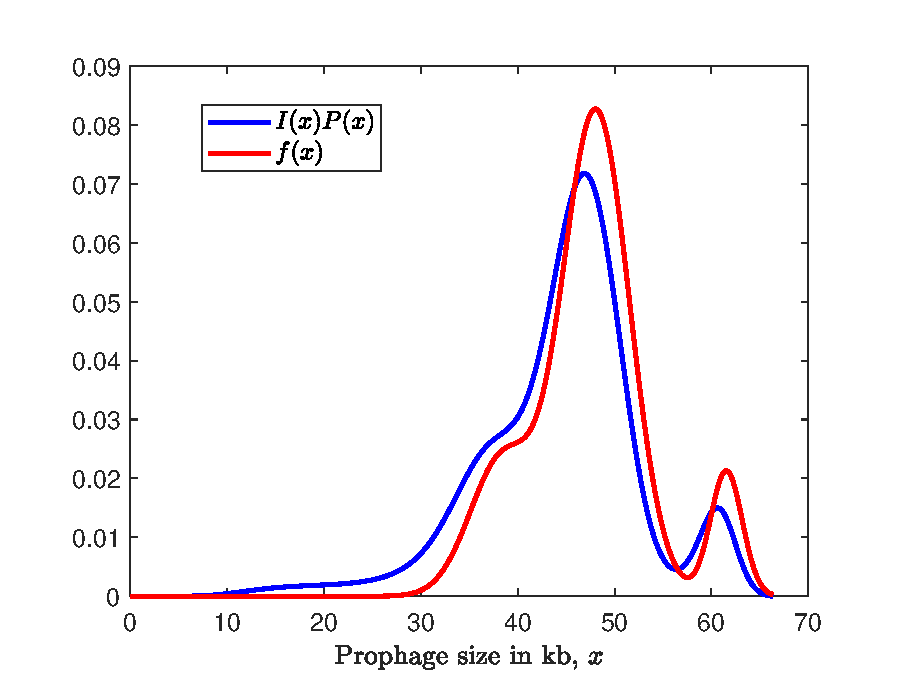
\includegraphics[scale=0.7]{IP.eps}
\caption[Comparison of best-fit $f(x)$ with the product $P(x)I(x)$.]{Comparison of best-fit $f(x)$ with the product $P(x)I(x)$; results shown for Data Set 1.}
\label{fig:IP}
\end{figure}
\addcontentsline{toc}{chapter}{Bibliography}
\bibliographystyle{apa}
\bibliography{refrence}